%!TEX root = ../report.tex

\todo{Purpose of the chapter
 Structure of the chapter
 Central themes of the chapter}

\section{System} {
\label{sec:system}

	%!TEX root = ../../../report.tex

\begin{figure}[H]
	\centering
	\figureborder{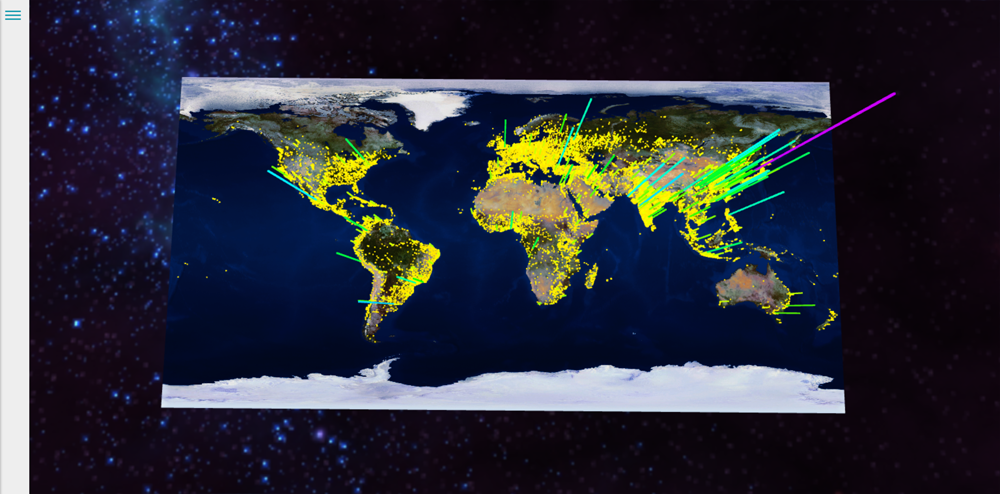
\includegraphics[width=\textwidth]{images/implementation/system/plane}}
	\caption{Population dataset on a plane surface.}
	\label{fig:plane_surface}
\end{figure}


	%!TEX root = ../../../report.tex

\begin{figure}[H]
	\centering
	\figureborder{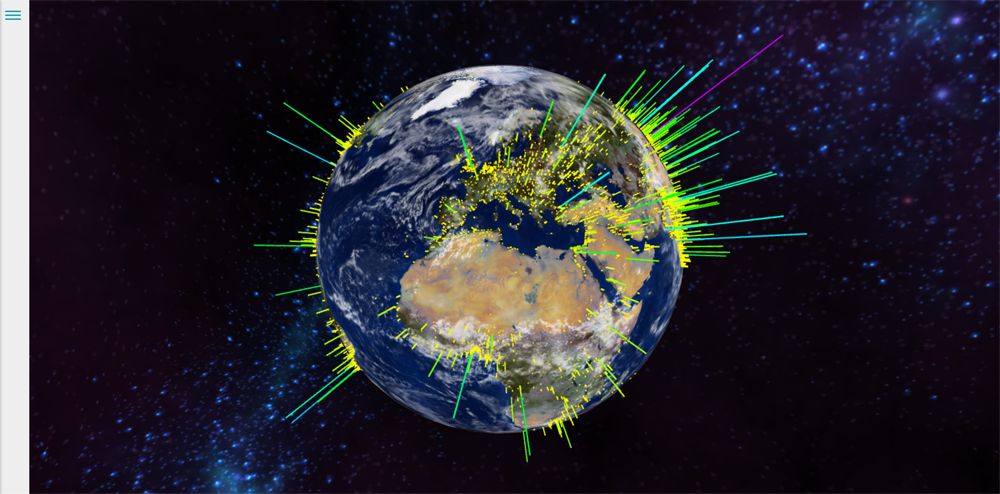
\includegraphics[width=\textwidth]{images/implementation/system/sphere}}
	\caption{Population dataset on a sphere surface.}
	\label{fig:sphere_surface}
\end{figure}


	%!TEX root = ../../../report.tex

\begin{figure}[H]
	\centering
	\figureborder{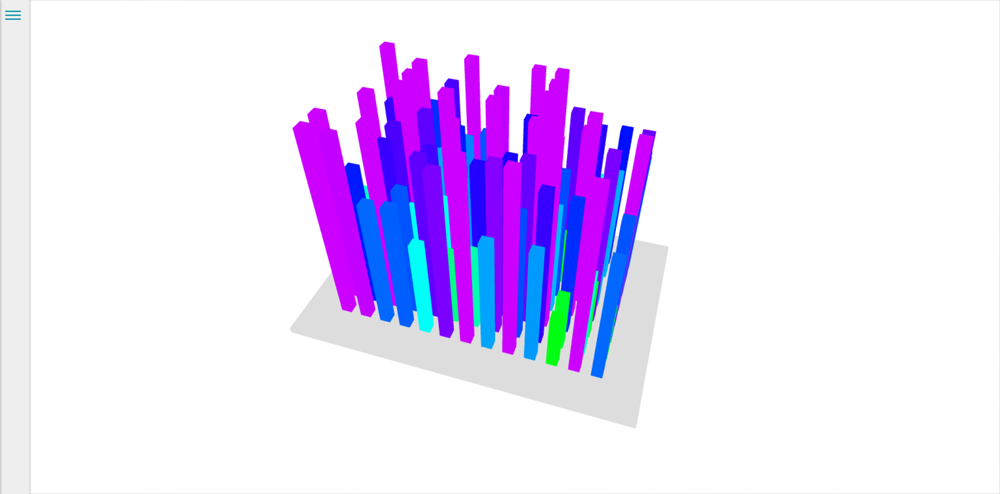
\includegraphics[width=\textwidth]{images/implementation/system/grid}}
	\caption{Student dataset on a grid surface.}
	\label{fig:grid_surface}
\end{figure}


	\todo{map to project outcomes}

	\todo{highlight integration and student data}
	
}

\section{Navigation} {
\label{sec:navigation}

	The navigation techniques that the user can interact with are: pan, rotate and zoom. This functionality was implemented in a single module and utilised mouse events to detect when the user was scrolling or pressing the left or right mouse button. It is important to note that Three.js uses a right-handed coordinate system, as shown in Figure~\ref{fig:threejs_coordinate_system}.

	%!TEX root = ../../report.tex

\begin{figure}[H]
	\centering
	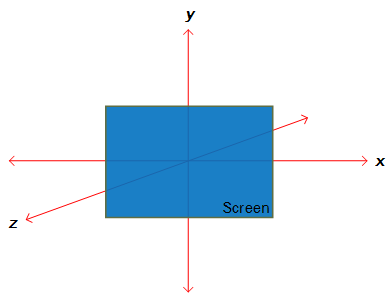
\includegraphics{images/implementation/threejs_coordinate_system}
	\caption[Three.js coordinate system]{Three.js coordinate system\protect\footnotemark.}
	\label{fig:threejs_coordinate_system}
\end{figure}

\footnotetext{\bibentry{microsoft2015threejs}}


	\subsection{Pan} {
	\label{sec:pan}

		This interaction is initiated when a \texttt{mousedown} event is fired on the canvas, followed by a \texttt{mousemove} event bound to the \texttt{window}. This simulates drag when pressing the left mouse button.

		As the user moves their pointer, the camera is translated in the x and y direction. This calculation relies on converting screen coordinates to world coordinates and normalising the value so it is a ratio of the viewport height, instead of both the width and height.

		Once the translation to the camera has been applied, the \texttt{origin} vector needs to be updated, which is used during rotation. An updated origin ensures there is no sudden movement when rotating, after panning the screen.

		Finally, when the user releases the left mouse button, a \texttt{mouseup} event is triggered which removes the event binding for \texttt{mousemove} on the \texttt{window}. 

	}

	\subsection{Rotate} {
	\label{sec:rotate}

		Rotation uses the same event chain as panning, except instead of listening to the left mouse click, it listens to the right.

		To rotate the camera, the cartesian coordinates need to be calculated from spherical coordinates, using the following formula in a right-handed mathetmatics system:

		%!TEX root = ../../report.tex

\begin{gather*}
	x = r\sin\phi\sin\theta \\
	y = r\cos\phi \\
	z = r\sin\phi\cos\theta
	\intertext{Where:}
	\begin{tabularx}{\textwidth}{@{}>{$}r<{$}@{\ :\ }X@{}}
		r & is the radial distance of the camera from the origin. \\
		\phi & is the polar angle, calculated by adding the delta phi angle with the angle from the y-axis. \\
		\theta & is the azimuthal angle, calculated by adding the delta theta angle with the angle from the z-axis around the y-axis. \\
	\end{tabularx}
\end{gather*}
	
	}

	\subsection{Zoom} {
	\label{sec:zoom}

		This navigation technique begins when a \texttt{wheel} event is triggered from the browser. A ratio of the delta value is taken and the camera is then translated by this amount.
	
	}

}

\section{Data point display} {
\label{sec:data_point_display}

	The data point displays were implemented by creating a \texttt{THREE.Mesh} that acts as a \texttt{Points} container for all \texttt{Point} meshes. The \texttt{Points} class is repsonsible for creating all of the data point displays, using the \texttt{Point} Backbone collection created and populated with information from the dataset during application startup.

	\todo{write about how the data displays were implemented - bunch of cubegeoms that get updated}

	\todo{mention flat - spherical projection for data points}

	%!TEX root = ../../report.tex

\begin{figure}[H]
	\captionsetup[subfigure]{aboveskip=-0.8em,belowskip=0.5em}
	\newcommand{\figurewidth}{0.5\textwidth}
	\begin{subfigure}[b]{\figurewidth}
        \figureborder{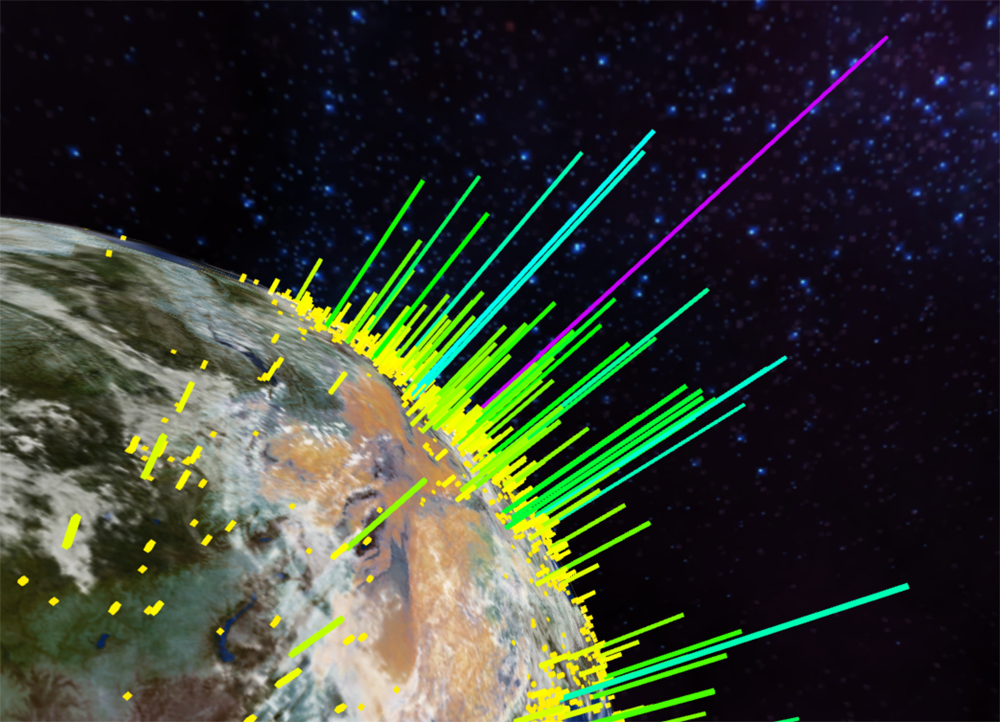
\includegraphics[width=\textwidth]{images/implementation/data_display/basic}}
		\caption{Basic shader data point display.}
		\label{fig:basic_shader}
	\end{subfigure}
	\begin{subfigure}[b]{\figurewidth}
		\figureborder{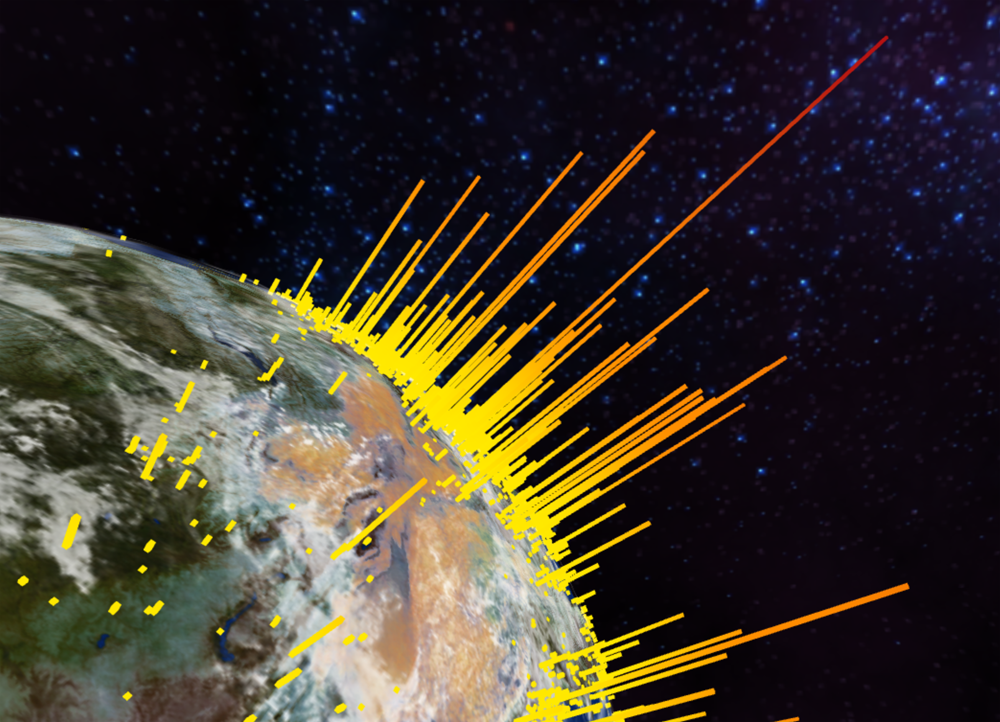
\includegraphics[width=\textwidth]{images/implementation/data_display/gradient}}
		\caption{Gradient shader data point display.}
		\label{fig:gradient_shader}
	\end{subfigure}
	\caption[Data point display types]{Types of data point displays.}
	\label{fig:data_point_displays}
\end{figure}


	% The development of these visualisations will involve using the established \href{http://threejs.org/docs/#Reference/Extras.Geometries/BoxGeometry}{BoxGeometry} that are available in Three.js.

}

\section{Information display} {
\label{sec:information_display}

	\todo{say how this was implemented - raycaster in requestanimframe, toggles one element to hide/show so nothing new in dom is added (more performant) recompiles the template}

	\todo{add for population and student data}

	%!TEX root = ../../report.tex

\begin{figure}[H]
	\centering
	\newcommand{\figurewidth}{0.4\textwidth}
	\centering
	\begin{subfigure}[b]{\figurewidth}
        \figureborder{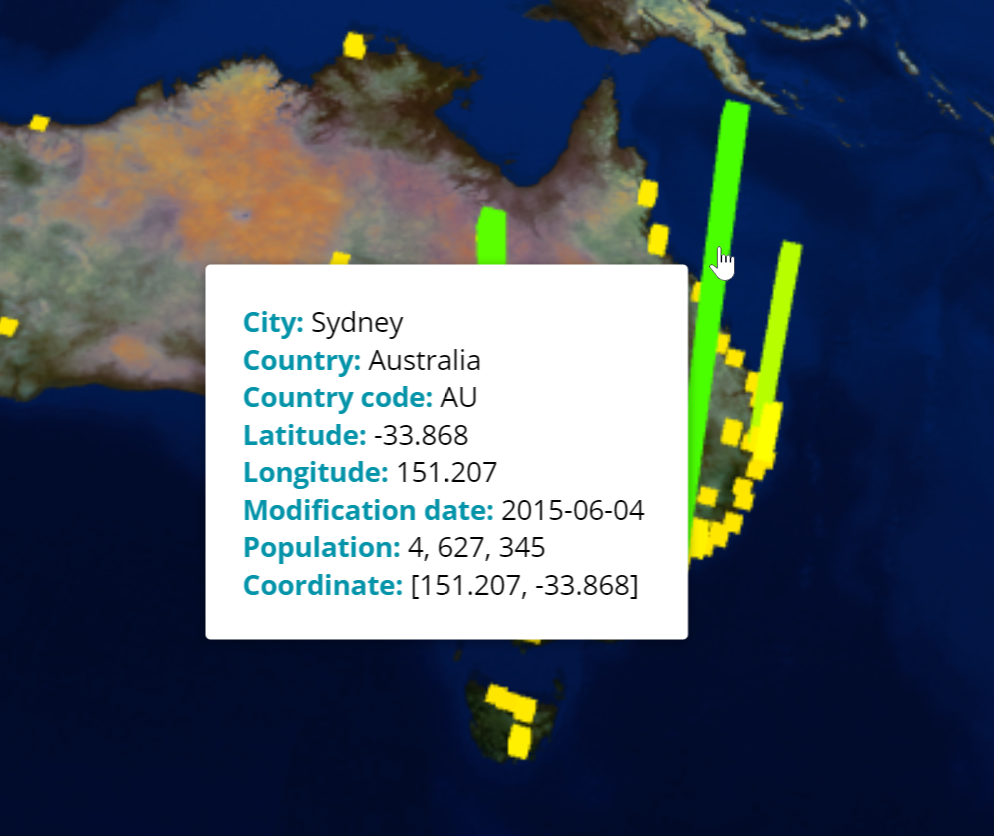
\includegraphics[width=\textwidth]{images/implementation/information_display/population}}
		\caption{Information display for population data.}
		\label{fig:information_display_population}
	\end{subfigure}
	\begin{subfigure}[b]{\figurewidth}
		\figureborder{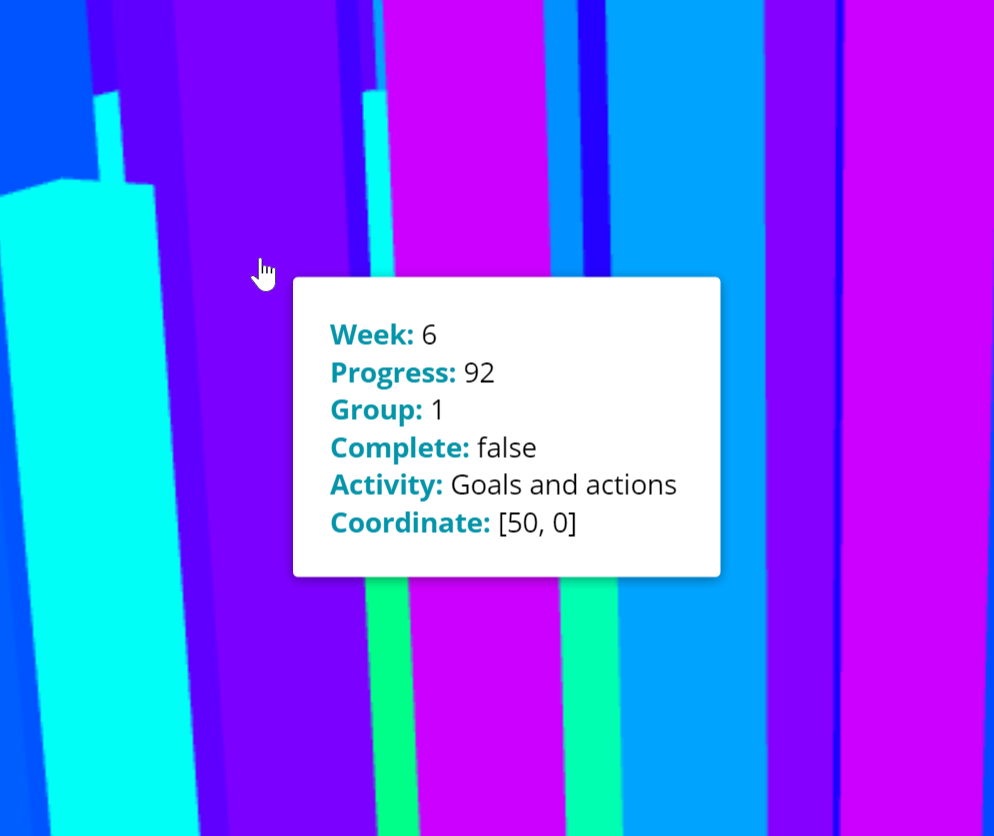
\includegraphics[width=\textwidth]{images/implementation/information_display/student}}
		\caption{Information display for student data.}
		\label{fig:information_display_student}
	\end{subfigure}
	\caption[Information display]{Information display hover effect.}
	\label{fig:information_display}
\end{figure}


}

\section{Skybox} {
\label{sec:skybox}

	\todo{write things}

}

\section{Drawer menu} {
\label{sec:drawer}

	The drawer menu is located on the left side of the system and is initially closed to maximise the visualisation viewing area. It has been built with pure CSS, using a checkbox that alters and transitions the position of the menu when the checkbox is checked. This interface has been shown in Figure~\ref{fig:drawer} below.

	%!TEX root = ../../report.tex

\begin{figure}[H]
	\newcommand{\figurewidth}{0.5\textwidth}
	\begin{subfigure}[b]{\figurewidth}
        \figureborder{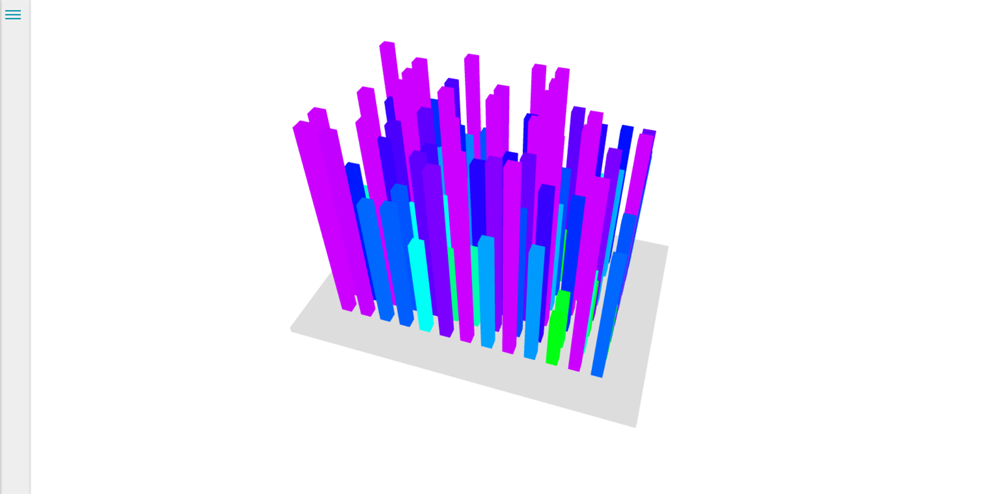
\includegraphics[width=\textwidth]{images/implementation/drawer/closed}}
		\caption{Closed drawer.}
		\label{fig:closed_drawer}
	\end{subfigure}
	\begin{subfigure}[b]{\figurewidth}
		\figureborder{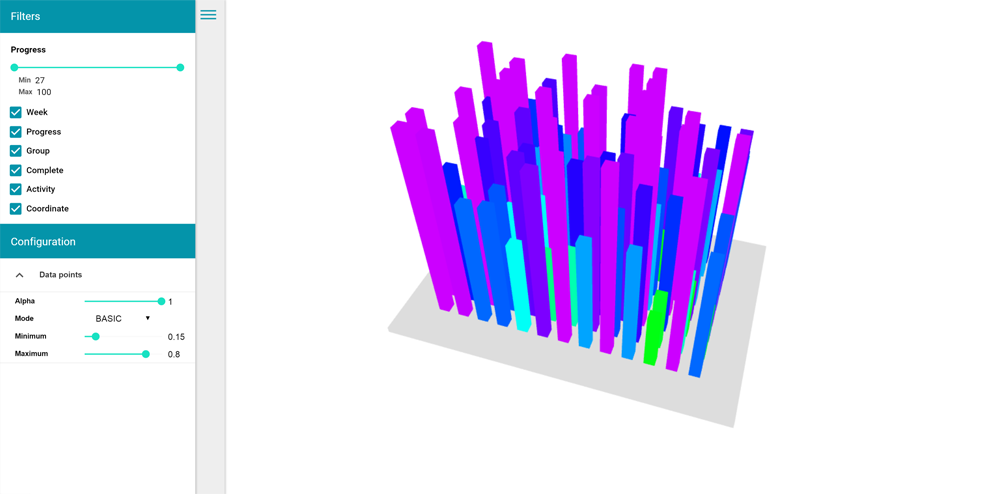
\includegraphics[width=\textwidth]{images/implementation/drawer/open}}
		\caption{Open drawer.}
		\label{fig:open_drawer}
	\end{subfigure}
	\caption{Drawer interface.}
	\label{fig:drawer}
\end{figure}


}

\section{Filtering} {
\label{sec:filtering_implementation}

	Filtering was implemented using an event-driven approach and a view controller for configuring the filters. This view controller comprises the slider and checkbox views, which were designed using Handlebars templates and populated with a Backbone model. The final design of this interface has been demonstrated in Figure~\ref{fig:filtering_interface}.

	%!TEX root = ../../../report.tex

\begin{wrapfigure}[13]{r}{0.4\textwidth}
	\captionsetup{aboveskip=0em}
	\vspace{-2.5em}
	\begin{center}
		\figureborder{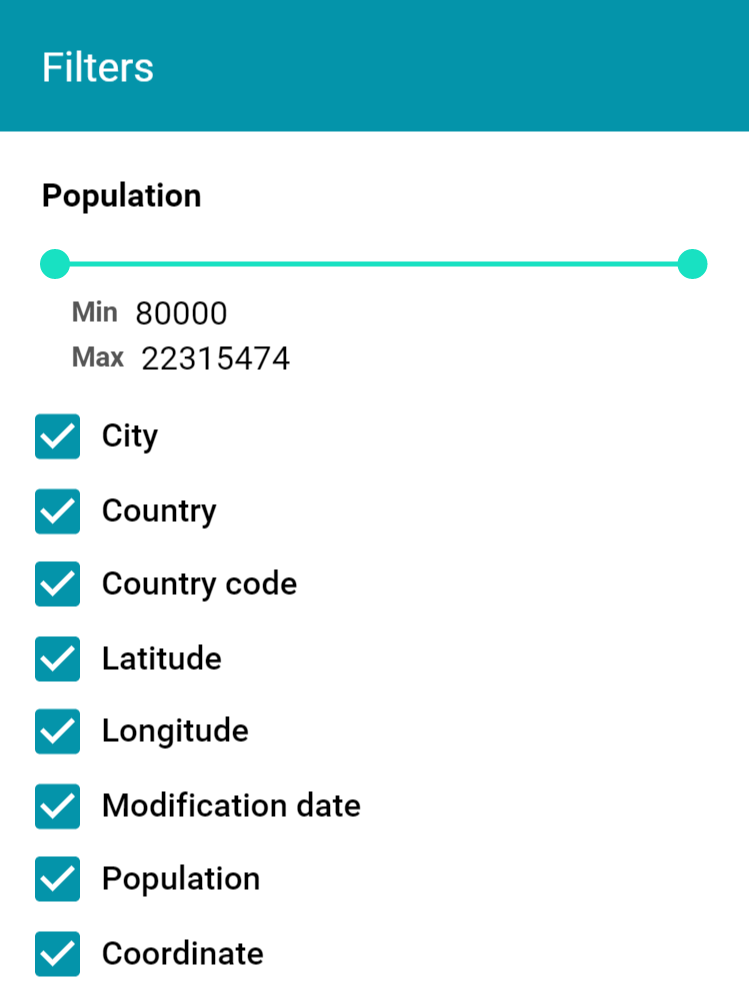
\includegraphics[width=0.4\textwidth]{images/implementation/filtering/interface}}
	\end{center}
	\caption[Filtering]{Filtering interface.}
	\label{fig:filtering_interface}
\end{wrapfigure}


	As a user adjusts the values in the slider, an \texttt{update} event is triggered. When this occurs, the event handler adjusts the minimum and maximum input to reflect the new slider widget values. Then, the Backbone collection that represents the data displays are filtered by calling the \texttt{filterBy} function with a filter function. This method is reposnsible for iterating through each model in the collection and determining if it should be filtered. A simple example of a filter function is:

	%!TEX root = ../../report.tex

\begin{lstlisting}
	function (model) {
		let value = model.get(property);
		return !(value > min && value <= max);
	}
\end{lstlisting}


	The above function utilises closure to check if the property associated with the slider is within the specified minimum and maximum bounds. If this function returns \texttt{true}, the model is added to a filtered collection. Once the collection has been iterated through, the \texttt{filterBy} function triggers a \texttt{filter} event with the filtered collection. This event is handled through other classes and ultimately modifies the visibility of the data display mesh based on the results of filtering.

	A similar process occurs when the user enters a value into the minimum or maximum inputs. A \texttt{keyup} event is bound to both inputs and a timer is in place to enforce a filtering delay. This delay ensures that filtering is processed as required, when the user has stopped typing, in order to reduce performance issues. When the user stops typing, the slider values are updated to match the input and filtering then proceeds as normal.

	As previously mentioned, the checkboxes represent what information is available to the user when hovering on a data display. The state of visibility for any given property is configured through a custom Handlebars helper method. This helper method is called when the information display template is updated, which is every time the user hovers on a data display. The helper method simply checks if a property is currently in a filtered list and displays the property when it is not a member of this list. So in order to configure the visibility of properties in the information display, a \texttt{change} event is bound to each chexkbox that updates the contents of the filtered list.

	The sequence of images displayed in Figure~\ref{fig:filtering_comparison} presents a comparison between the results of filtering for both data displays and information displays. From this, it can be seen that the user activities outlined in Section~\ref{sec:user_actions} have the potential to be fulfilled more quickly when there is less data to navigate through.

	%!TEX root = ../../../report.tex

\begin{figure}[H]
	\captionsetup[subfigure]{aboveskip=8pt,belowskip=8pt}
	\newcommand{\figurewidth}{0.5\textwidth}
	\begin{subfigure}[b]{\figurewidth}
		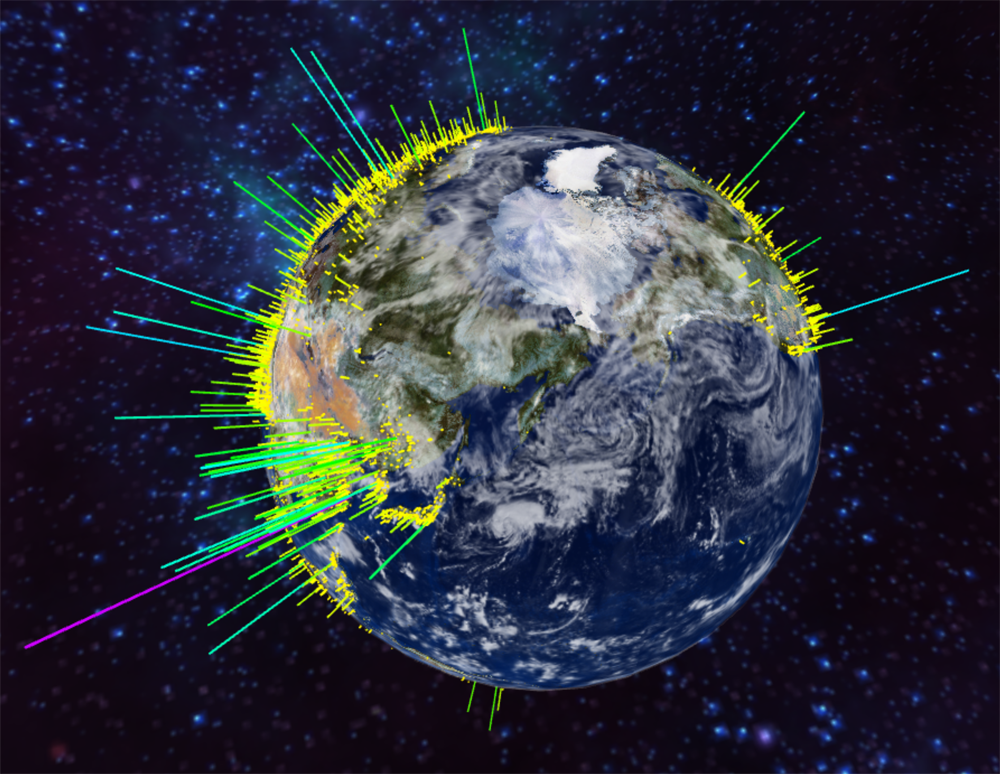
\includegraphics[width=\textwidth]{images/implementation/filtering/magnitude_before}
		\caption{Before filtering the magnitude.}
		\label{fig:before_filtering_magnitude}
	\end{subfigure}
	\begin{subfigure}[b]{\figurewidth}
		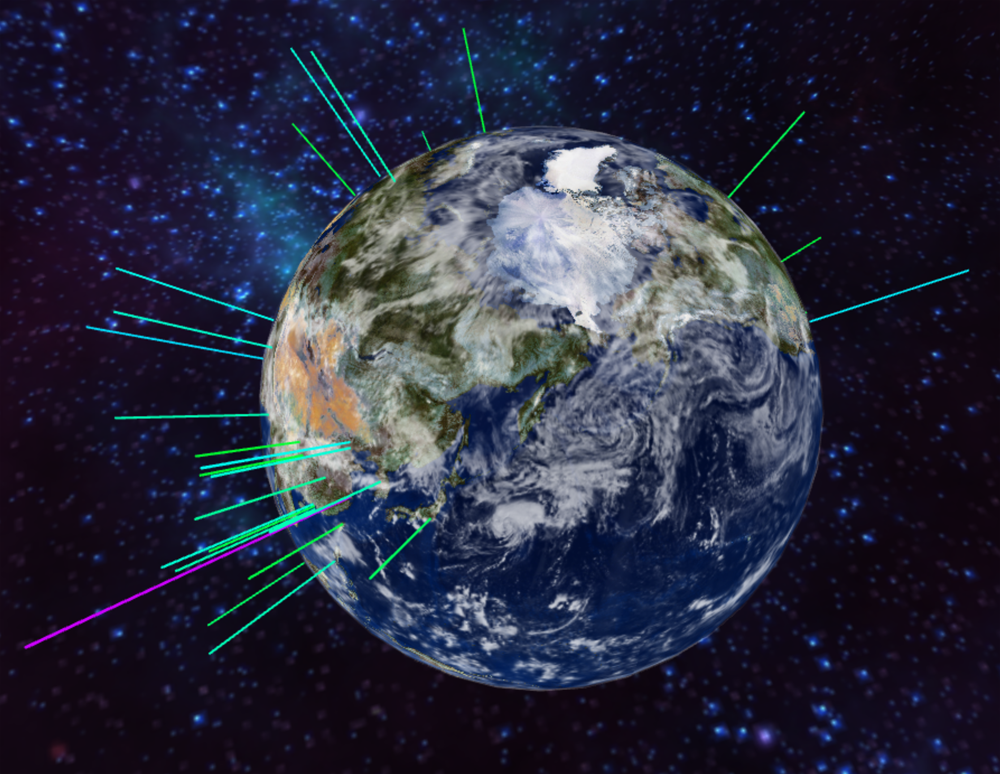
\includegraphics[width=\textwidth]{images/implementation/filtering/magnitude_after}
		\caption{After filtering the magnitude}
		\label{fig:after_filtering_magnitude}
	\end{subfigure}
	\begin{subfigure}[b]{\figurewidth}
		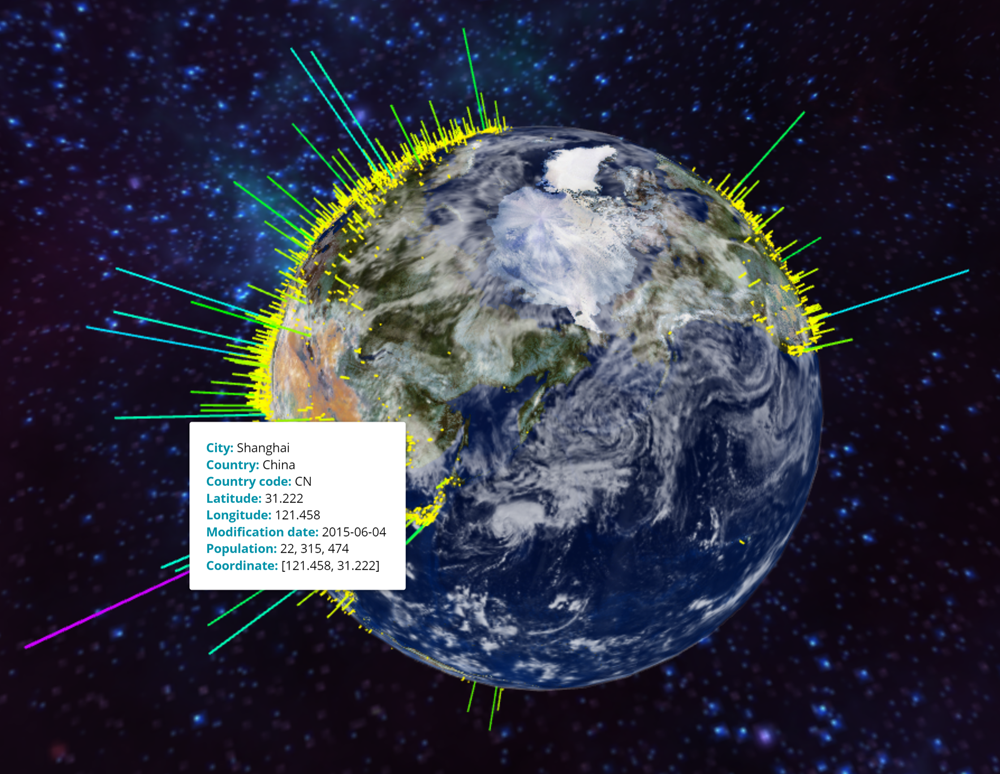
\includegraphics[width=\textwidth]{images/implementation/filtering/information_before}
		\caption{Before filtering information.}
		\label{fig:before_filtering_information}
	\end{subfigure}
	\begin{subfigure}[b]{\figurewidth}
		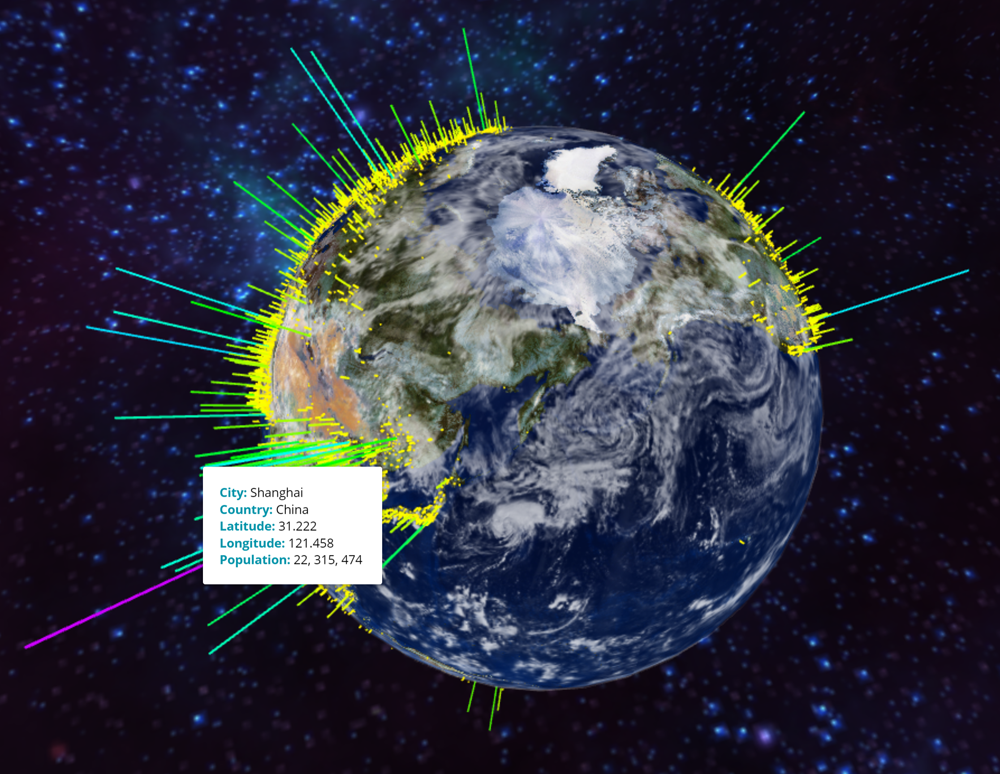
\includegraphics[width=\textwidth]{images/implementation/filtering/information_after}
		\caption{After filtering information.}
		\label{fig:after_filtering_information}
	\end{subfigure}
	\caption[Filtering comparison]{Filtering comparison.}
	\label{fig:filtering_comparison}
\end{figure}


}

\section{Configuration} {
\label{sec:configuration_implementation}

	Real-time configurations are best achieved by using shaders. Shaders are computer programs that perform shading on a graphics processing unit (GPU), making them highly efficient and well suited to parallel processing~\footnote{\bibentry{gerdelan2014shaders}}. Three.js provides abstracted materials that use shaders in the background, but this method does not easily facilitate highly customisable configurations or filter effects. Therefore, custom shaders were designed and implemented for the system to maximise efficiency and flexibility. An example of the available effects that were implemented in the system is shown in Figure~\ref{fig:shaders}.

	%!TEX root = ../../report.tex

\begin{figure}[H]
	\captionsetup[subfigure]{aboveskip=-0.8em,belowskip=0.5em}
	\newcommand{\figurewidth}{0.5\textwidth}
	\begin{subfigure}[b]{\figurewidth}
        \figureborder{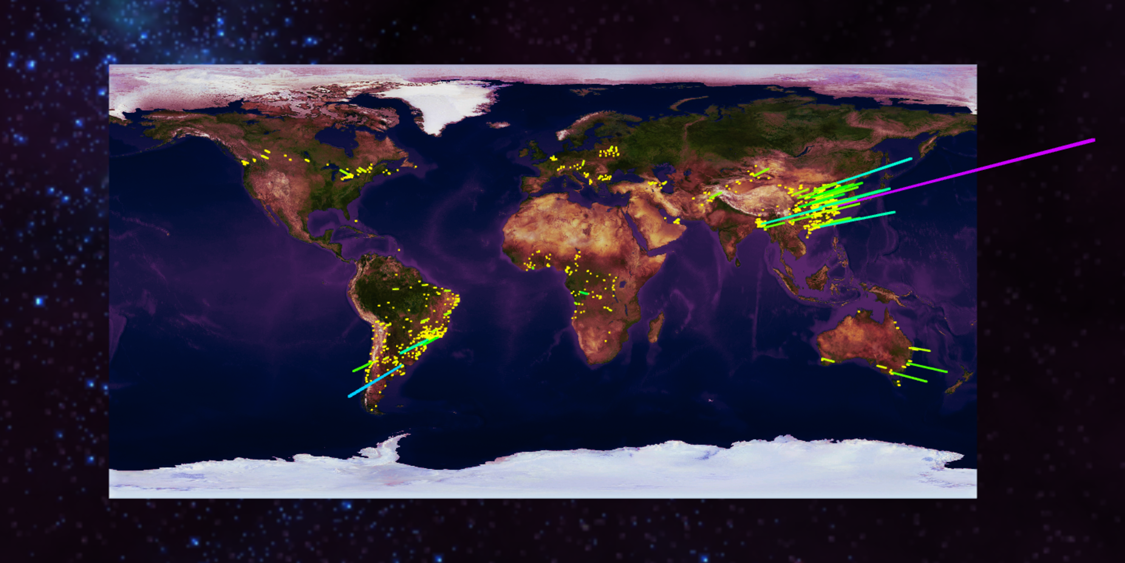
\includegraphics[width=\textwidth]{images/implementation/shaders/red}}
		\caption{Red midtone filter effect.}
		\label{fig:red_midtone}
	\end{subfigure}
	\begin{subfigure}[b]{\figurewidth}
		\figureborder{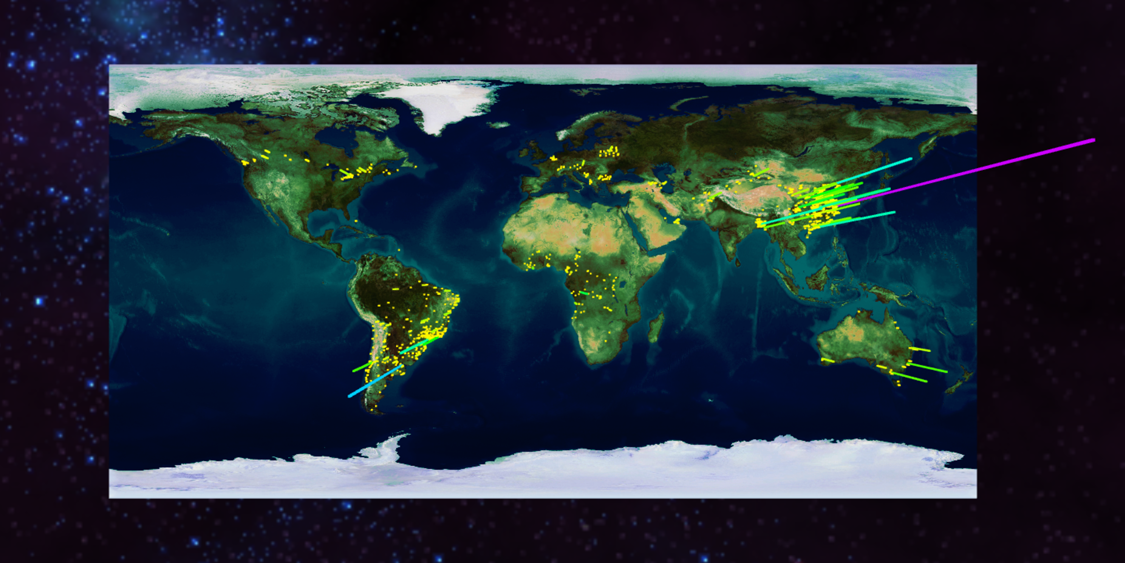
\includegraphics[width=\textwidth]{images/implementation/shaders/green}}
		\caption{Green midtone filter effect.}
		\label{fig:green_midtone}
	\end{subfigure}
	\begin{subfigure}[b]{\figurewidth}
		\figureborder{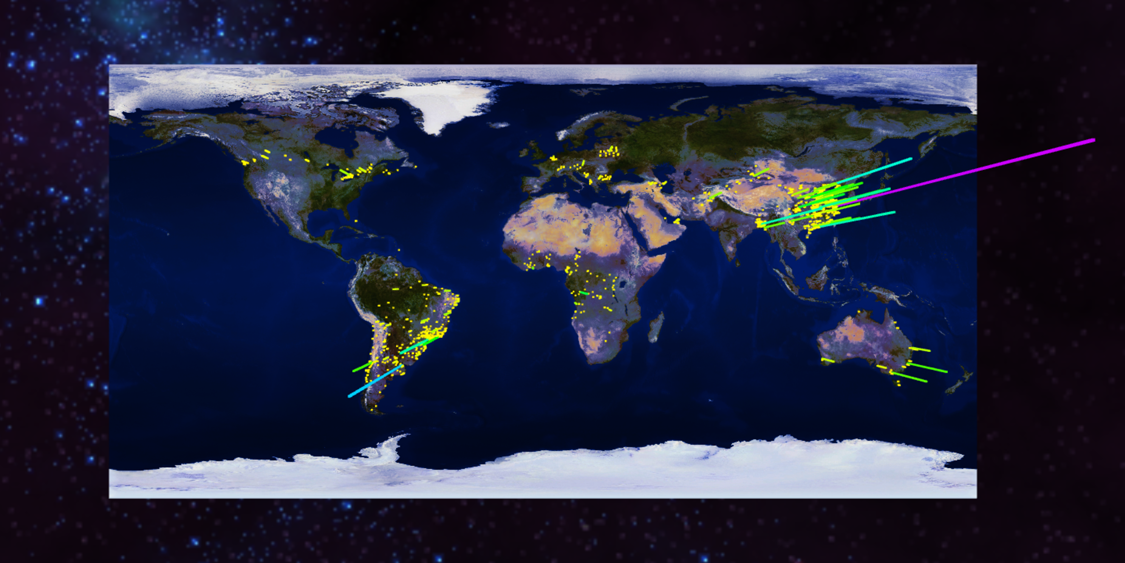
\includegraphics[width=\textwidth]{images/implementation/shaders/blue}}
		\caption{Blue midtone filter effect.}
		\label{fig:blue_midtone}
	\end{subfigure}
	\begin{subfigure}[b]{\figurewidth}
		\figureborder{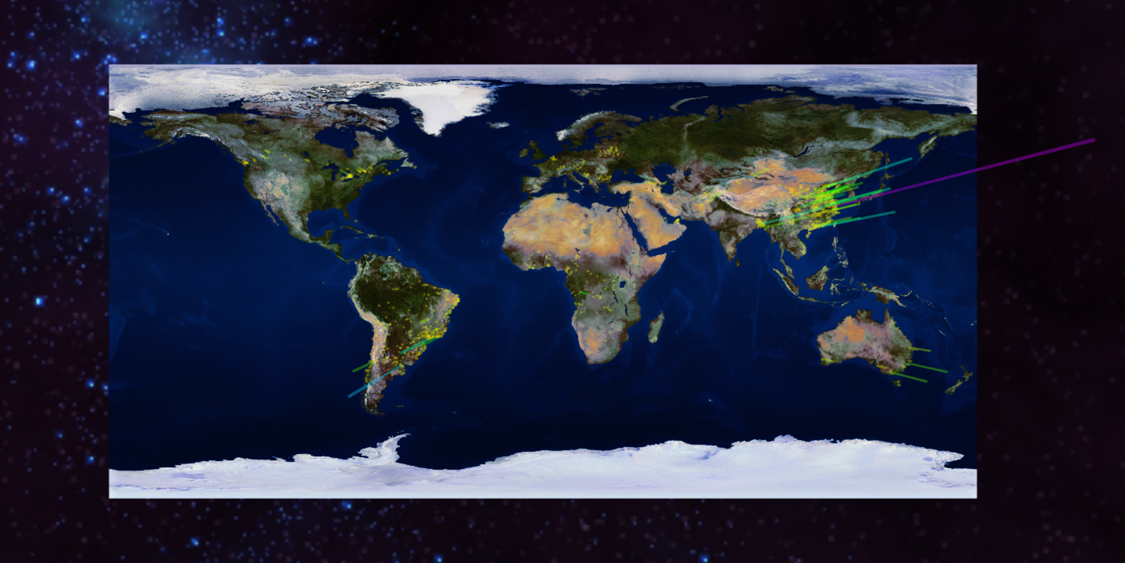
\includegraphics[width=\textwidth]{images/implementation/shaders/opacity}}
		\caption{Opacity filter effect.}
		\label{fig:opacity_filter}
	\end{subfigure}
	\begin{subfigure}[b]{\figurewidth}
		\figureborder{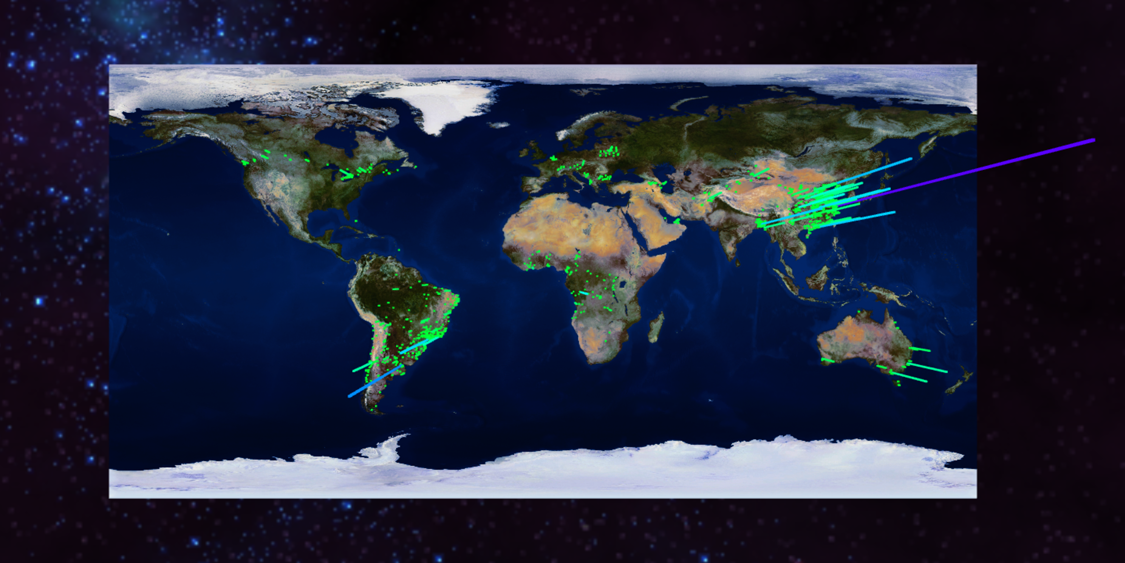
\includegraphics[width=\textwidth]{images/implementation/shaders/basic}}
		\caption{Alternate HSV colour range.}
		\label{fig:hsv_colour}
	\end{subfigure}
	\begin{subfigure}[b]{\figurewidth}
		\figureborder{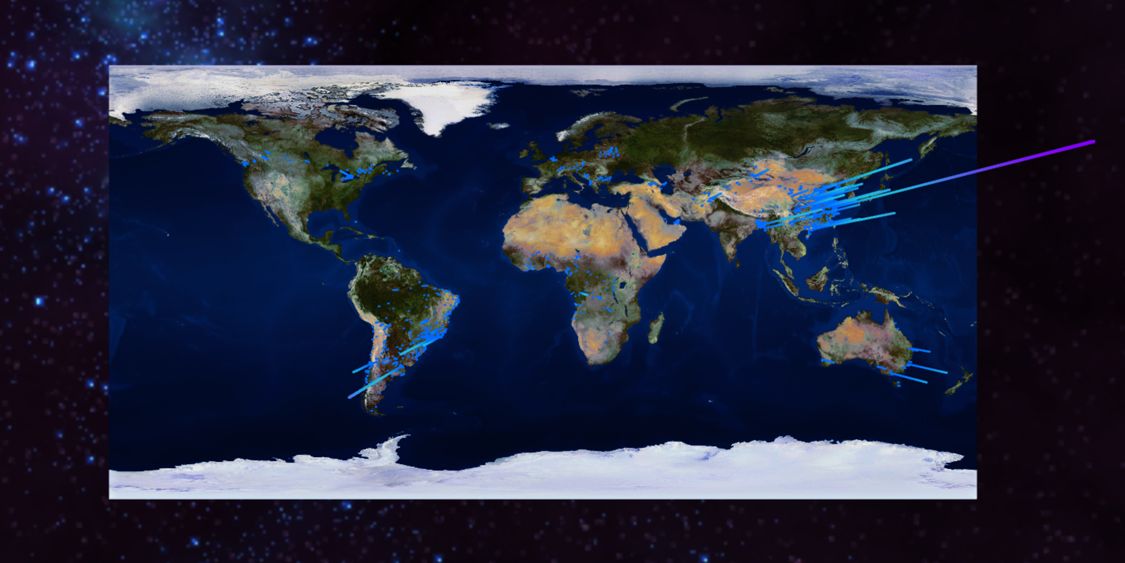
\includegraphics[width=\textwidth]{images/implementation/shaders/gradient}}
		\caption{Alternate gradient colour scheme.}
		\label{fig:gradient_colour}
	\end{subfigure}
	\caption[Shaders]{Available shader filter effects.}
	\label{fig:shaders}
\end{figure}


	These configurations can be adjusted in real-time with \href{http://workshop.chromeexperiments.com/}{dat.GUI}, a lightweight GUI for changing JavaScript variables in real-time. This tool is easy to use, setup and can modify shader uniforms automatically or by implementing \texttt{onChange} event handlers. dat.GUI can constrain input data and provides widgets for modifying values, colours and combo boxes. While this tool is great for modifying data on the fly, it has an outdated interface that does not always adapt well to particular colour schemes and designs. For this reason, the dat.GUI styles were modified to seamlessly integrate with the current system and the Material Design standards. The differences in design can be compared in Figure~\ref{fig:dat_gui} below.

	%!TEX root = ../../report.tex

\begin{figure}[H]
	\newcommand{\figurewidth}{0.4\textwidth}
	\newcommand{\figureheight}{7cm}
	\centering
	\begin{subfigure}[b]{\figurewidth}
        \figureborder{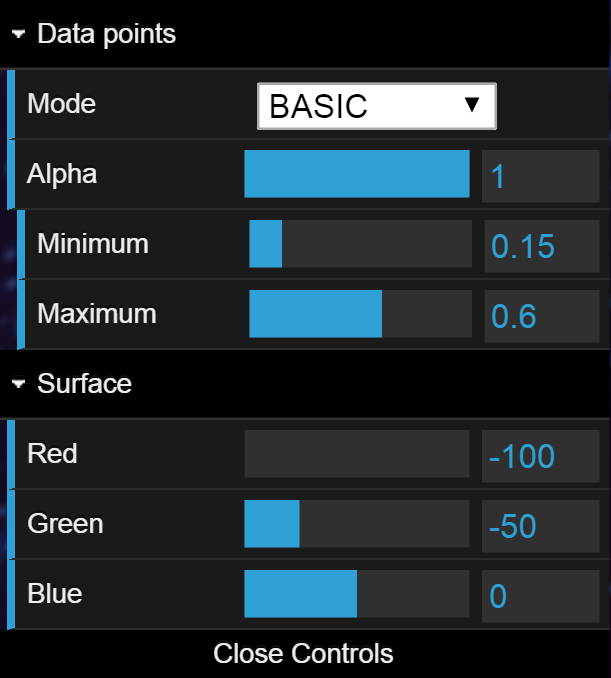
\includegraphics[width=\textwidth,height=\figureheight]{images/implementation/dat_gui/before}}
		\caption{Original dat.GUI interface.}
		\label{fig:dat_gui_before}
	\end{subfigure}
	\begin{subfigure}[b]{\figurewidth}
		\figureborder{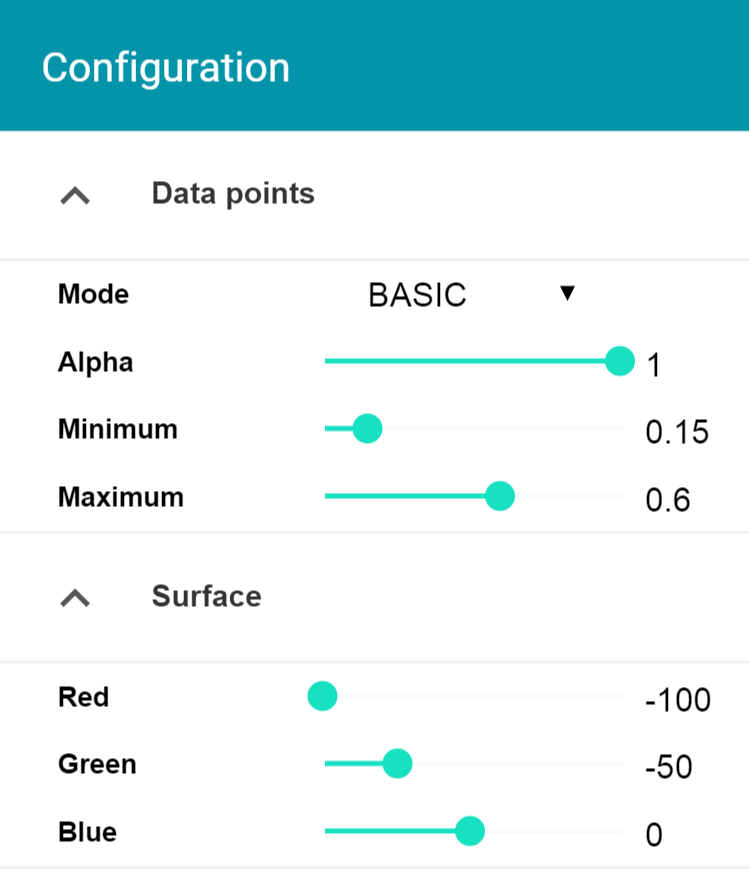
\includegraphics[width=\textwidth,height=\figureheight]{images/implementation/dat_gui/after}}
		\caption{dat.GUI interface after custom styling.}
		\label{fig:dat_gui_after}
	\end{subfigure}
	\caption[dat.GUI interface]{dat.GUI interface.}
	\label{fig:dat_gui}
\end{figure}


	The design for these configurations were continually refined during implementation. Initially, the dat.GUI sliders were to remain unchanged. However, these sliders proved to be inconsistent in regards to the colour scheme and filter design. Furthermore, the bold folder colours were eventually removed to reflect drawer layouts that conform to using light navigation colours, hover effects, and left floated icons.

}

\section{Evaluations} {
\label{sec:evaluations}

	\todo{performance slow with large data mention filtering and configuration}

	\todo{map to project outcomes and user issues here and reflect everything}

}
